\input{../YKY-preamble.tex}
% \usepackage[no-math]{fontspec}
% \setmainfont[BoldFont=Alibaba_Sans_Regular.otf,ItalicFont=Alibaba_Sans_Light_Italic.otf]{Alibaba_Sans_Light.otf}

\usepackage[backend=biber]{biblatex}
\bibliography{../AGI-book}

\usepackage[active,tightpage]{preview}		% for continuous page(s)
\renewcommand{\PreviewBorder}{0.5cm}
\renewcommand{\thempfootnote}{\arabic{mpfootnote}}

\usepackage[absolute,overlay]{textpos}		% for page number on upper left corner

\usepackage{color}
% \usepackage{mathtools}
\usepackage[hyperfootnotes=false]{hyperref}

% \usepackage[backend=biber,style=numeric]{biblatex}
% \bibliography{../AGI-book}
% \renewcommand*{\bibfont}{\footnotesize}

\usetikzlibrary{shapes}
% \usepackage[export]{adjustbox}	% ??
\usepackage{verbatim} % for comments
% \usepackage{newtxtext,newtxmath}	% Times New Roman font

% \titleformat{\subsection}[hang]{\bfseries\large\color{blue}}{}{0pt}{} 
% \numberwithin{equation}{subsection}

\newcommand{\underdash}[1]{%
	\tikz[baseline=(toUnderline.base)]{
		\node[inner sep=1pt,outer sep=10pt] (toUnderline) {#1};
		\draw[dashed] ([yshift=-0pt]toUnderline.south west) -- ([yshift=-0pt]toUnderline.south east);
	}%
}%

\newcommand\reduline{\bgroup\markoverwith{\textcolor{red}{\rule[-0.5ex]{2pt}{0.4pt}}}\ULon}

%\DeclareSymbolFont{symbolsC}{U}{txsyc}{m}{n}
%\DeclareMathSymbol{\strictif}{\mathrel}{symbolsC}{74}
%\DeclareSymbolFont{AMSb}{U}{msb}{m}{n}
%\DeclareSymbolFontAlphabet{\mathbb}{AMSb}
%\setmathfont{lmroman17-regular.otf}
\DeclareMathOperator*{\argmin}{arg\,min}
\DeclareMathOperator*{\argmax}{arg\,max}

% \usepackage[most]{tcolorbox}
%\tcbset{on line, 
%	boxsep=4pt, left=0pt,right=0pt,top=0pt,bottom=0pt,
%	colframe=red,colback=pink,
%	highlight math style={enhanced}
%}
%\newcommand{\atom}{\vcenter{\hbox{\tcbox{....}}}}

\let\oldtextbf\textbf
\renewcommand{\textbf}[1]{\textcolor{blue}{\oldtextbf{#1}}}

\newcommand{\logic}[1]{{\color{violet}{\textit{#1}}}}
\newcommand{\underconst}{\includegraphics[scale=0.5]{../2020/UnderConst.png}}
\newcommand{\KBsymbol}{\vcenter{\hbox{\includegraphics[scale=1]{../KB-symbol.png}}}}
\newcommand{\token}{\vcenter{\hbox{\includegraphics[scale=1]{token.png}}}}
\newcommand{\proposition}{\vcenter{\hbox{\includegraphics[scale=0.8]{proposition.png}}}}

\begin{document}

\begin{preview}

\title{\vspace{-1.5cm} \bfseries\color{blue}{\LARGE Measuring the ``size'' of hypothesis spaces over $\mathbb{R}$ from the perspective of No Free Lunch}}

\author{Yan King Yin} % Your name
% \date{\vspace{-2cm}} % Date, can be changed to a custom date

\maketitle

\setcounter{section}{-1}
\newcounter{mypage}
\setcounter{mypage}{0}

% (1) Circled page number on upper left corner
\begin{textblock*}{5cm}(2.1cm,2.3cm) % {block width} (coords) 
{\color{red}{\large \textcircled{\small \themypage}}}
\addtocounter{mypage}{1}
\end{textblock*}

\begin{minipage}{\textwidth}
\setlength{\parskip}{0.4\baselineskip}

\section{Motivating example}

\begin{equation}
\vcenter{\hbox{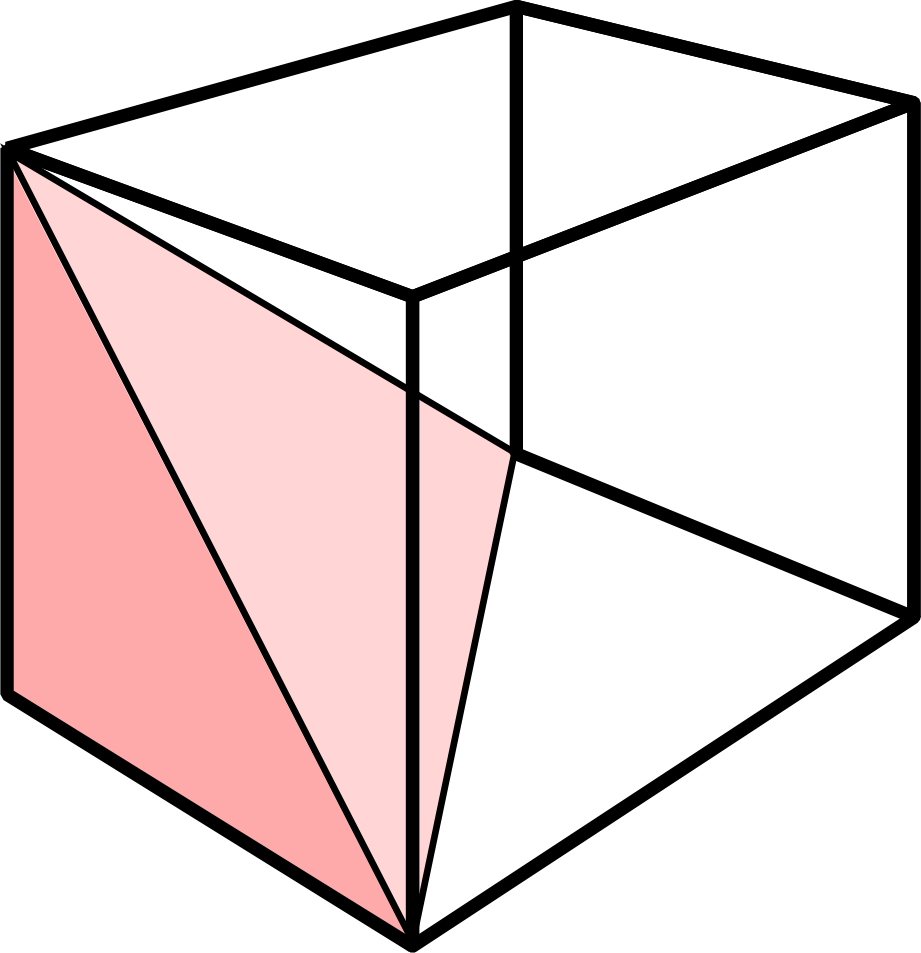
\includegraphics[scale=0.7]{cube-corner.png}}}
\end{equation}

The \textbf{input space} is $X = \mathbb{R}^n = n$-dimensional hypercube.  Permutation symmetry implies that only one corner of the hypercube need be considered, this is the \textbf{fundamental domain}.  The \textbf{volume} of this domain over the entire hypercube shrinks exponentially as $n$ grows, which appears to suggest that this symmetry is very significant for efficiency consideration.  We want to quantify the notion of this efficiency.

We want to compare the \textbf{hypothesis spaces} $A$ and $B$:  $A$ = unconstrained, fully-connected neural network with $L$ layers and $N$ total weights.  The parameter space $A = \Theta_A = \mathbb{R}^N$.  Case $B$ = symmetric neural network with a special structure but nonetheless its parameter space is also of the form $B = \Theta_B = \mathbb{R}^M$.

\begin{equation}
\vcenter{\hbox{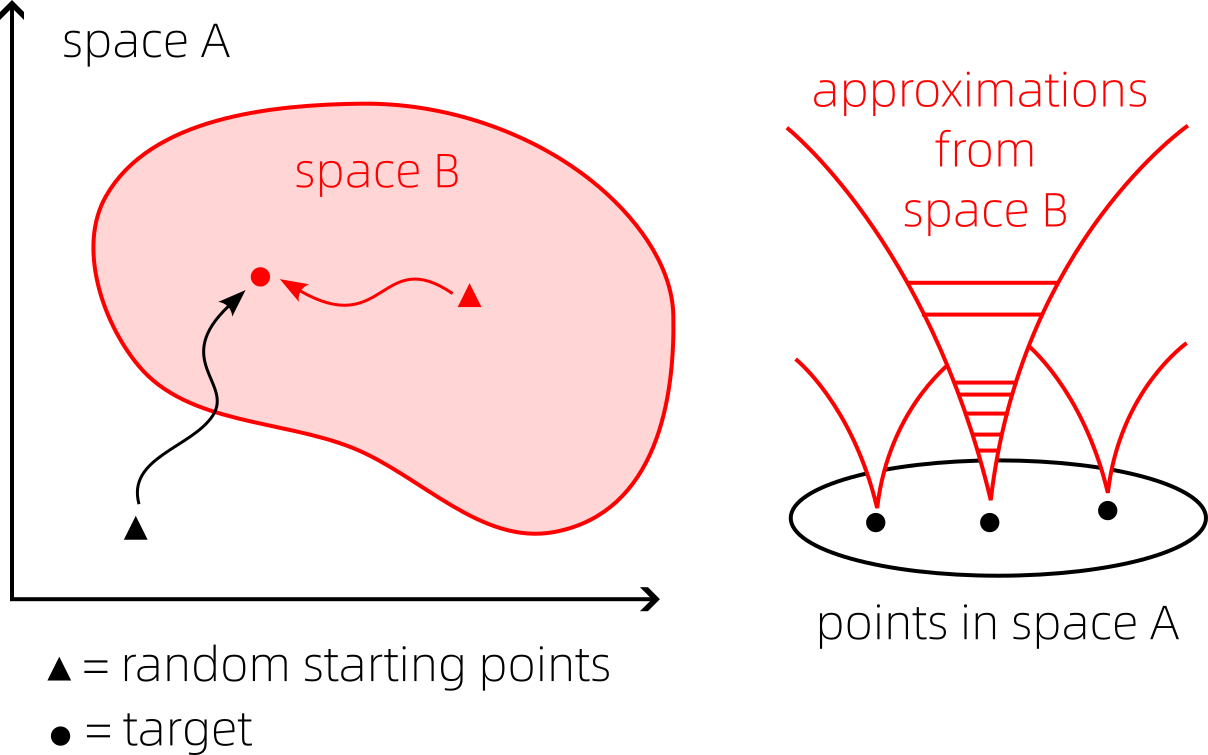
\includegraphics[scale=0.7]{no-free-lunch.png}}}
\end{equation}

It's easier to consider $A$ and $B$ as both embedded in an ambient function space $\mathcal{H}$ that is ``fine'' enough to contain all points of $A$ and $B$:
\begin{equation}
\vcenter{\hbox{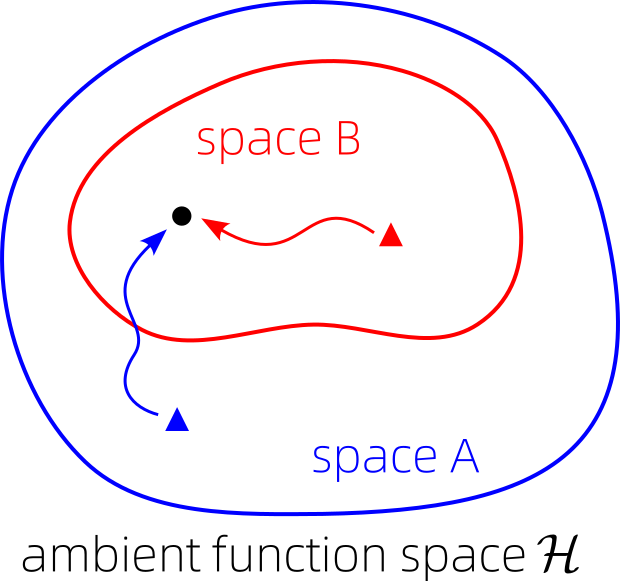
\includegraphics[scale=0.7]{no-free-lunch-2.png}}} \qquad
\begin{aligned}
& \text{Embeddings:} \\
& {\color{blue}\Theta_A \hookrightarrow} \; \mathcal{H} \\
& {\color{red}\Theta_B \hookrightarrow} \; \mathcal{H} 
\end{aligned}
\end{equation}

We also need a measure of the ``roughness'' of the landscapes $A$ and $B$ in the function space $\mathcal{H}$.  The objective function $ J = J( f(x_i; \Theta) - y_i ) $.

\end{minipage}
\end{preview}

\begin{preview}
\begin{textblock*}{5cm}(2.1cm,2.3cm) % {block width} (coords) 
	{\color{red}{\large \textcircled{\small \themypage}}}
	\addtocounter{mypage}{1}
\end{textblock*}

\begin{minipage}{\textwidth}
	\setlength{\parskip}{0.4\baselineskip}

\section{This}

\begin{itemize}
	\item Here
\end{itemize}

\end{minipage}
\end{preview}

\begin{preview}
\begin{textblock*}{5cm}(2.1cm,2.3cm) % {block width} (coords) 
{\color{red}{\large \textcircled{\small \themypage}}}
\addtocounter{mypage}{1}
\end{textblock*}

\begin{minipage}{\textwidth}
\setlength{\parskip}{0.4\baselineskip}

\section{This}

\begin{itemize}
	\item Here
\end{itemize}

\end{minipage}
\end{preview}

\begin{preview}
\begin{textblock*}{5cm}(2.1cm,2.3cm) % {block width} (coords) 
	{\color{red}{\large \textcircled{\small \themypage}}}
	\addtocounter{mypage}{1}
\end{textblock*}

\begin{minipage}{\textwidth}
	\setlength{\parskip}{0.4\baselineskip}

\section{This}

\begin{itemize}
	\item Here
\end{itemize}

\end{minipage}
\end{preview}

\end{document}
